\documentclass[border=10pt]{standalone}
\usepackage{ifthen}
\usepackage{tikz}
\usetikzlibrary{
  arrows,
  arrows.meta,
}
\usepackage{pgfplots}
\usepgfplotslibrary{
    fillbetween,
}
\usetikzlibrary[calc]

\begin{document}

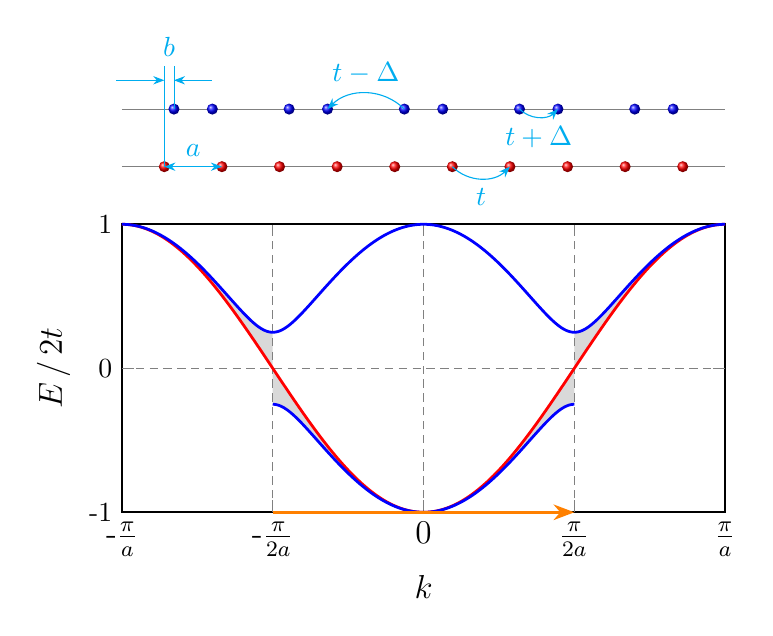
\begin{tikzpicture}
    [
        x=0.48in, y=0.72in,
    ]
    \begin{axis}
    [
        x=0.48in, y=0.72in,
        declare function = {
            % Hopping Integral in TB
            t = 1.0;
            % Band Gap after Peierls Dimerization
            g = 0.25;
            % Band dispersion in TB
            b1(\x) = -t * cos(deg(\x));
            % Band dispersion after Dimerization within TB
            b2(\x) = sqrt(
                t^2 * cos(deg(\x))^2
                +
                g^2 * sin(deg(\x))^2
            );
        },
        % width=3.2in, height=2.4in,
        xmin=-pi, xmax=pi,
        ymin=-1, ymax=1,
        xtick = {-pi, -pi/2, 0, pi/2, pi},
        xticklabels = {-$\frac{\pi}{a}$, -$\frac{\pi}{2a}$, $0$, $\frac{\pi}{2a}$, $\frac{\pi}{a}$},
        ytick = {-1, 0, 1},
        yticklabels = {-$1$, $0$, $1$},
        xlabel = {$k$},
        ylabel = {$E \,/\, 2t$},
        ylabel near ticks,
        xlabel style= {font=\large},
        xticklabel style= {font=\large},
        ylabel style= {font=\large},
        axis line style = {line width=0.8pt},
        clip = false,
    ]
    \addplot [densely dashed, color=gray, line width=0.5pt] coordinates {(-pi/2, -1) (-pi/2, 1)};
    \addplot [densely dashed, color=gray, line width=0.5pt] coordinates {(pi/2, -1) (pi/2, 1)};
    \addplot [densely dashed, color=gray, line width=0.5pt] coordinates {(0, -1) (0, 1)};
    \addplot [densely dashed, color=gray, line width=0.5pt] coordinates {(-pi, 0) (pi, 0)};

    \addplot [name path=A, samples=300, domain=-pi:pi,  line width=1.0pt, color=red] { b1(x)};
    \addplot [name path=B, samples=300, domain=-pi:pi, line width=1.0pt, color=blue] { b2(x)};
    \addplot [name path=C, samples=300, domain=-pi/2:pi/2, line width=1.0pt, color=blue] {-b2(x)};
    % \addplot [name path=B, samples=300, domain=-pi:-pi/2, line width=1.0pt, color=blue] { b2(x)};
    % \addplot [name path=C, samples=300, domain=pi/2:pi, line width=1.0pt, color=blue] { b2(x)};
    % \addplot [name path=D, samples=300, domain=-pi/2:pi/2, line width=1.0pt, color=blue] {-b2(x)};

    \addplot [gray!30] fill between [
        of = C and A,
        soft clip={domain=-pi/2:pi/2}
    ];
    \addplot [gray!30] fill between [
        of = B and A,
        soft clip={domain=-pi:-pi/2}
    ];
    \addplot [gray!30] fill between [
        of = B and A,
        soft clip={domain=pi/2:pi}
    ];

    \draw[line width=1pt, color=orange, ->, >=Stealth] (axis cs: -pi/2, -1) -- (axis cs: pi/2, -1);

    % draw the atoms
    \draw[help lines] (axis cs: -pi, 1.4) -- (axis cs: pi, 1.4);
    \foreach \ii in {-5,...,4}{
        \pgfmathparse{\ii*0.6 + 0.3}
        \edef\temp{\noexpand\shade[ball color=red] (axis cs: \pgfmathresult, 1.4) circle (2.0pt);}
        \temp
    }

    \draw[help lines] (axis cs: -pi, 1.8) -- (axis cs: pi, 1.8);
    \foreach \ii in {-5,-3,...,4}{
        \pgfmathparse{\ii*0.6 + 0.3 + 0.1}
        \edef\temp1{\noexpand\shade[ball color=blue] (axis cs: \pgfmathresult, 1.8) circle (2.0pt);}
        \temp1
        \pgfmathparse{\ii*0.6 + 0.9 - 0.1}
        \edef\temp2{\noexpand\shade[ball color=blue] (axis cs: \pgfmathresult, 1.8) circle (2.0pt);}
        \temp2
    }
    % the hoppign integral
    \draw[out=-45, in=-135, cyan, -{Stealth[length=4pt]}]
    (axis cs: 0.3, 1.4)
    to
    node[pos=0.5, below] {$t$}
    (axis cs: 0.9, 1.4);

    \draw[out=-45, in=-135, cyan, -{Stealth[length=4pt]}]
    (axis cs: 1.0, 1.8)
    to
    node[pos=0.5, below] {$t + \Delta$}
    (axis cs: 1.4, 1.8);
    
    \draw[out=135, in=45, cyan, -{Stealth[length=4pt]}]
    (axis cs: -0.2, 1.8)
    to
    node[pos=0.5, above] {$t - \Delta$}
    (axis cs: -1.0, 1.8);

    \draw[{Stealth[length=4pt]}-{Stealth[length=4pt]}, cyan]
    (axis cs: -2.7, 1.4)
    --
    node[pos=0.5, above] {$a$}
    (axis cs: -2.1, 1.4);

    \draw[help lines, cyan] (axis cs: -2.7, 1.4) -- (axis cs: -2.7, 2.1);
    \draw[help lines, cyan] (axis cs: -2.6, 1.8) -- (axis cs: -2.6, 2.1);
    \draw[cyan, {Stealth[length=4pt]}-] (axis cs: -2.7, 2.0) -- (axis cs: -3.2, 2.0);
    \draw[cyan, {Stealth[length=4pt]}-] (axis cs: -2.6, 2.0) -- (axis cs: -2.2, 2.0);
    \node[above, cyan] at (axis cs: -2.65, 2.1) {$b$};
    \end{axis}
\end{tikzpicture}

\end{document}
